\section{Overview}

\begin{figure}[H]
        \centering 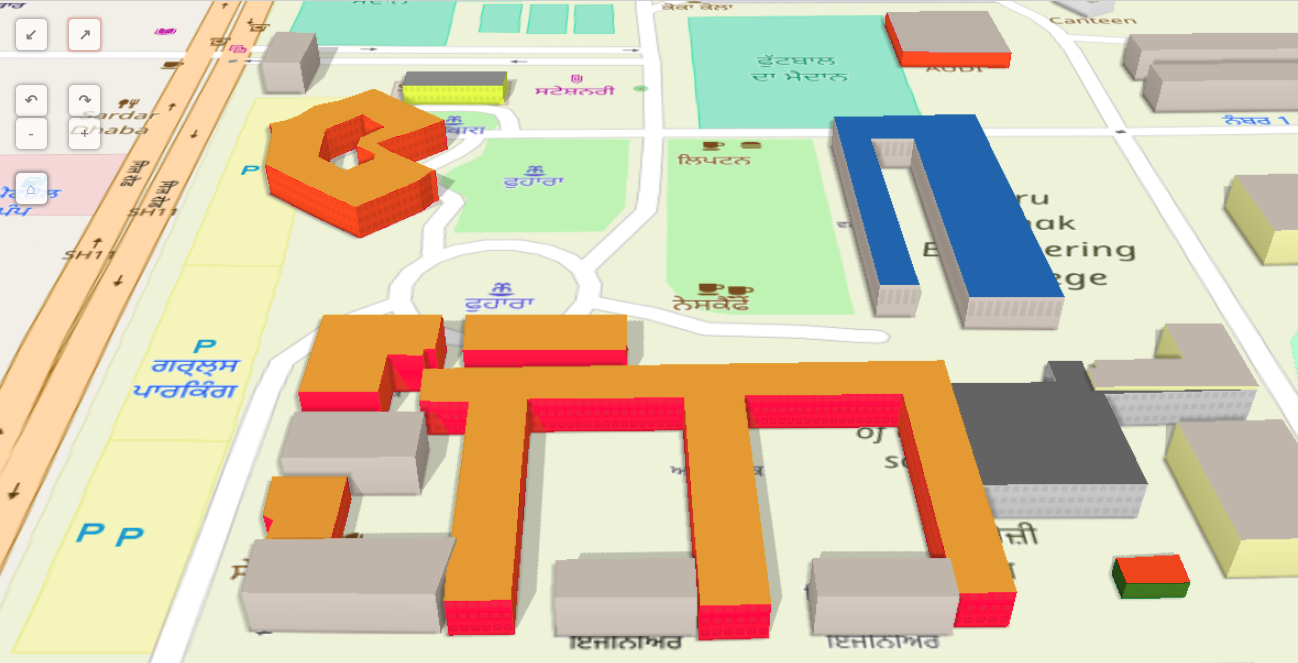
\includegraphics[scale=0.31]{input/images/osm_building.png}
        \caption{OpenStreetMap}
        \label{fig:openscadlogo}
\end{figure}

OpenStreetMap (OSM) is an open-source, free web-based software, owned by you, the contributors.OpenStreetMap is an online open data platform to collect the world's geographic data based on the Wikipedia model of crowdsourcing. The project started in 2004 by Steve Coast and is now governed by the non profit OpenStreetMap Foundation based in the UK.\\ 


OpenStreetMap is a free editable map of the whole world. It is made by people like you.” Which
means the database will always be subject to the whims, experimentation, and mistakes of the
community. This is precisely OSM’s strength since, among other things, it allows our data to
quickly accommodate changes in the physical world.


By making your system an OSM tile server not only you can edit the map but can use it offline
also. You can change the styling of the map like color of the roads fonts style and amny more as
per your requirments.\\


The core part of OSM is implemented using Mapnik library and database for rendering, mod\_tile and slippy
for web interface. Bash Shell Scripting has been used to automate the installation.


My training being not based on particular language or technology, different type of open-source softwares and technologies are
used in this project and many during my training which are not used in this
project like CGI (for web interface through c++).

\section{Existing System}
Geographical data (geo data) is not free in many parts of the world.If you collect data from Google Maps in this way, you are creating a "derived work". Any such data retains the copyright conditions of the original. In practice, this means your data is subject to the licensing fees, and contractual restrictions, of these map providers. That's exactly what OpenStreetMap is trying to avoid. The data is copyrighted and owned by multiple organisations like the Ordnance Survey. Google/whoever just licenses it. If we were to use it, we'd have to pay for it.\\ 

In areas where there are no such data sources (most areas) we have to start from a blank slate, and head out there to survey the streets ourselves. Despite starting from scratch, we have achieved a good level of completion in many places.  

"Also, you may not use Google Maps in a manner which gives you or any other person access to mass downloads or bulk feeds of numerical latitude and longitude coordinates."

{\bf {Limitations of the existing system }}
\begin{itemize}
\item We can't edit the maps.

\item Data may be inaccurate.

\item They are costly.

\item Can't create own map server.

\item Mass downloads or bulk feeds of numerical latitude and longitude coordinates is sometime impossible.
\end{itemize}

\section{User Requirement Analysis}
User Requirements Analysis for a software system is a complete description of the require-
ments of the User. It includes functional Requirements and Non-functional Requirements.
Non-functional requirements are requirements which impose constraints on the design or im-
plementation.

\begin{itemize}
\item{\bf Purpose}: OpenStreetMap (OSM) is an open collaborative project to  create a free editable map of the world and the main purpose of this project is to:
\begin{enumerate}
\item  To  create a free editable map of the world.
\item To gather location data  using GPS, local knowledge, and other free sources of information and upload it.
\item  To encourage the growth, development and distribution of free geospatial data.
\item  To provide geospatial data for anyone to use and share.
\item Reduce the time for analysis.
\item The OpenStreetMap Foundation is an international not-for-profit organization supporting, but not controlling, the OpenStreetMap Project.
\end{enumerate}
\end{itemize}
\subsection{Users of the System}


\begin{enumerate}
\item Provides beautiful GUI (Graphical User Interface) for GNE Tour and animations.
\item A full editing history is stored for each user.
\item Provide on-line way to analysis so that individual does not have to
install anything.
\item Users can attach Wikipedia-like edit summaries to their edits, and there is a History tab on the main page that shows recent edits to the selected area.
\item The user can download the data in *.pbf or *.osm file format.
\item Both techinal and non-technical users can use OSM.
\item User can make own OSM tile server.
\item User can run script for automatic installation.
\item They can search places with ease.

\end{enumerate}


\subsection{Functional Requirements}
\begin{itemize}
\item {\bf Specific Requirements}: This phase covers the whole requirements
for the system. After understanding the system we need the input data
to the system then we watch the output and determine whether the output
from the system is according to our requirements or not. So what we have
to input and then what we'll get as output is given in this phase. This
phase also describe the software and non-function requirements of the
system.
\item {\bf Input Requirements of the System}
\begin{enumerate}
\item Guess points and name of the places.
\item Precision
\item Required point at which value is to be found
\item Knowledge of latitude and longitude.
\end{enumerate}
\vskip 0.5cm
\item {\bf Output Requirements of the System}
\begin{enumerate}
\item Final output of the location of the particulaar area.
\item Shops, restaurants and many more are represented through icon and images.
\end{enumerate}
\vskip 0.5cm
\item {\bf Special User Requirements}
\begin{enumerate}
\item Taking bulk input values through html forms.
\end{enumerate}
\vskip 0.5cm
\item {\bf Software Requirements}
\begin{enumerate}
\item Programming language: C++, Python
\item software: \LaTeX{}
\item Web Languages: php, javascript, html
\item Database: Postgresql
\item Documentation: Doxygen 1.8.3
\item Text Editor: Vim
\item Operating System: Ubuntu 14.04 or 15.10
\item Revision System: Git

\end{enumerate}
\vskip 0.5cm
\subsection{Non functional requirements}
\begin{enumerate}
\item Scalability: System should be able to handle a number of users.
For e.g., handling around thousand users at the same time.
\item Usability: Simple user interfaces that a layman can understand.
\item Speed: Processing input should be done in reasonable time
 i.e. we can say maximum 24 hrs.
\end{enumerate}
\end{itemize}



\section{Feasibility Study}
Feasibility study aims to uncover the strengths and weaknesses of
a project. In its simplest term, the two criteria to judge feasibility
are cost required and value to be attained. As such, a well-designed
feasibility analysis should provide a historical background of the
project, description of the project or service, details of the
operations and management and legal requirements.\\

The objective of the feasibility study is to establish the reasons for developing the software that is acceptable to users, adaptable to change and conformable to established standards.\\
Objectives of feasibility study are listed below:
\begin{itemize}
        \item To analyze whether the software will meet organizational requirements.
        \item To determine whether the software can be implemented using the current technology and within the specified budget and schedule.
        \item To determine whether the software can be integrated with other existing software.
\end{itemize}


Generally, feasibility
analysis precedes technical development and project implementation.
These are some feasibility factors by which we can determine that
the project is feasible or not:

\subsection{Types of Feasibility Study}
Various types of feasibility that are commonly considered include technical feasibility, economic feasibility, and behaviourial feasibility.

\subsubsection{Technical Feasibility}
The Technical feasibility assessment is focused on gaining an understanding of the present technical resources of the organization and their applicability to the expected needs of the proposed system. It is an evaluation of the hardware and software and how it meets the need of the proposed system. This assessment is based on an outline design of system requirements, to determine whether the company has the technical expertise to handle completion of the project.\\

 This whole project is based on Open
                Source Environment and is part of an open source software which would be deployed on any OS.


The project is developed such that the necessary functions and performance are achieved within the constraints. The project is developed within latest technology. Through the technology may become obsolete after some period of time, due to the fact that never version of same software supports older versions, the system may still be used. So there are minimal constraints involved with this project. The system has been developed using Java the project is technically feasible for development.

Democratic Maps is technically feasible as it is built up using various open source technologies and it can run on any platform.

\subsubsection{Economic Feasibility}
The purpose of the economic feasibility assessment is to determine the positive economic benefits to the organization that the proposed system will provide. It includes quantification and identification of all the benefits expected. This assessment typically involves a cost/ benefits analysis.\\

Economic feasibility is the cost and logistical outlook for a business project or endeavor. Prior to embarking on a new venture, most businesses conduct an economic feasibility study, which is a study that analyzes data to determine whether the cost of the prospective new venture will ultimately be profitable to the company. Economic feasibility is sometimes determined within an organization, while other times companies hire an external company that specializes in conducting economic feasibility studies for them.\\

In addition, it is necessary to consider the benefits that can be achieved by developing the software. Software is said to be economically feasible if it focuses on the issues listed below.
\begin{itemize}
	\item Cost incurred on software development to produce long-term gains for an organization.
	\item Cost required to conduct full software investigation (such as requirements elicitation and requirements analysis).
	\item Cost of hardware, software, development team, and training.
\end{itemize}


Since the system is developed as part of project work, there is no manual cost to spend for the proposed system. Also all the resources are already available, it give an indication of the system is economically possible for development.

\subsubsection{Behavioral Feasibility}
Behavioral feasibility assesses the extent to which the required software performs a series of steps to solve business problems and user requirements. It is a measure of how well the solution of problems or a specific alternative solution will work in the organization. It is also measure of how people feel about the system. If the system is not easy to operate, than operational process would be difficult. The operator of the system should be given proper training. The system should be made such that the user can interface the system without any problem.\\

Operational feasibility is a measure of how well a proposed system solves the problems, and takes advantage of the opportunities identified during scope definition and how it satisfies the requirements identified in the requirements analysis phase of system development. The operational feasibility assessment focuses on the degree to which the proposed development projects fits in with the existing business environment and objectives with regard to development schedule, delivery date, corporate culture, and existing business processes.\\

To ensure success, desired operational outcomes must be imparted during design and development. These include such design-dependent parameters such as reliability, maintainability, supportability, usability, producibility, disposability, sustainability, affordability and others. These parameters are required to be considered at the early stages of design if desired operational behaviors are to be realized. A system design and development requires appropriate and timely application of engineering and management efforts to meet the previously mentioned parameters. A system may serve its intended purpose most effectively when its technical and operating characteristics are engineered into the design. Therefore, operational feasibility is a critical aspect of systems engineering that needs to be an integral part of the early design phasesThis feasibility is dependent on human resources (software development team) and involves visualizing whether the software will operate after it is developed and be operative once it is installed. Operational feasibility also performs the following tasks.\\

\begin{itemize}
	\item Determines whether the problems anticipated in user requirements are of high priority.
	\item Determines whether the solution suggested by the software development team is acceptable.
	\item Analyzes whether users will adapt to a new software.
	\item Determines whether the organization is satisfied by the alternative solutions proposed by the software development team.
\end{itemize}

This includes the following questions:
\begin{itemize}
	\item The project provids sufficient support for the users as the tiles are already stored in system.
	\item The proposed system would not cause any harm as it is running on a server rather than a client side.
	\item The project would be beneficial because it satisfies the objectives when developed and installed. All behavioral aspects are considered carefully and conclude that the project is behaviorally feasible.
\end{itemize}

\section{Objectives of Project }
The main objective of this project is to help GNE freshers to locate the places like labs, Admin Block, TCC etc from phone or laptop easily. The map is provided in Punjabi language. They can easily search the place by typing in the search button. In order to entertain them, the projects includes animations, GNE Tour and lot more. 
\begin{enumerate}
\item The map includes 3-D View with the shadows of buildings.
\item Styling of the map by adding international boundary of India.
\item Automation for making the system an OSM tile server.
\end{enumerate}

